\documentclass[12pt,letterpaper]{article}
\usepackage{preamble}

\newcommand\course{Linear Control Theory}
\newcommand\hwnumber{2}
\newcommand\userID{Daniil Manakovskiy}
\newcommand\userGroup{BS18-02}

\begin{document}
Variant: C
\section*{Question 2}
\label{Q:2}
\textit{Step-by-step calculations are present on the following page}
\begin{enumerate}[leftmargin=!,labelindent=5pt]
    \item 
    The total transfer function is
    \begin{equation*}
        \frac{100s^2+120s+20}{150s^5+325s^4-16s^3-220s^2-197s-42}
    \end{equation*}

    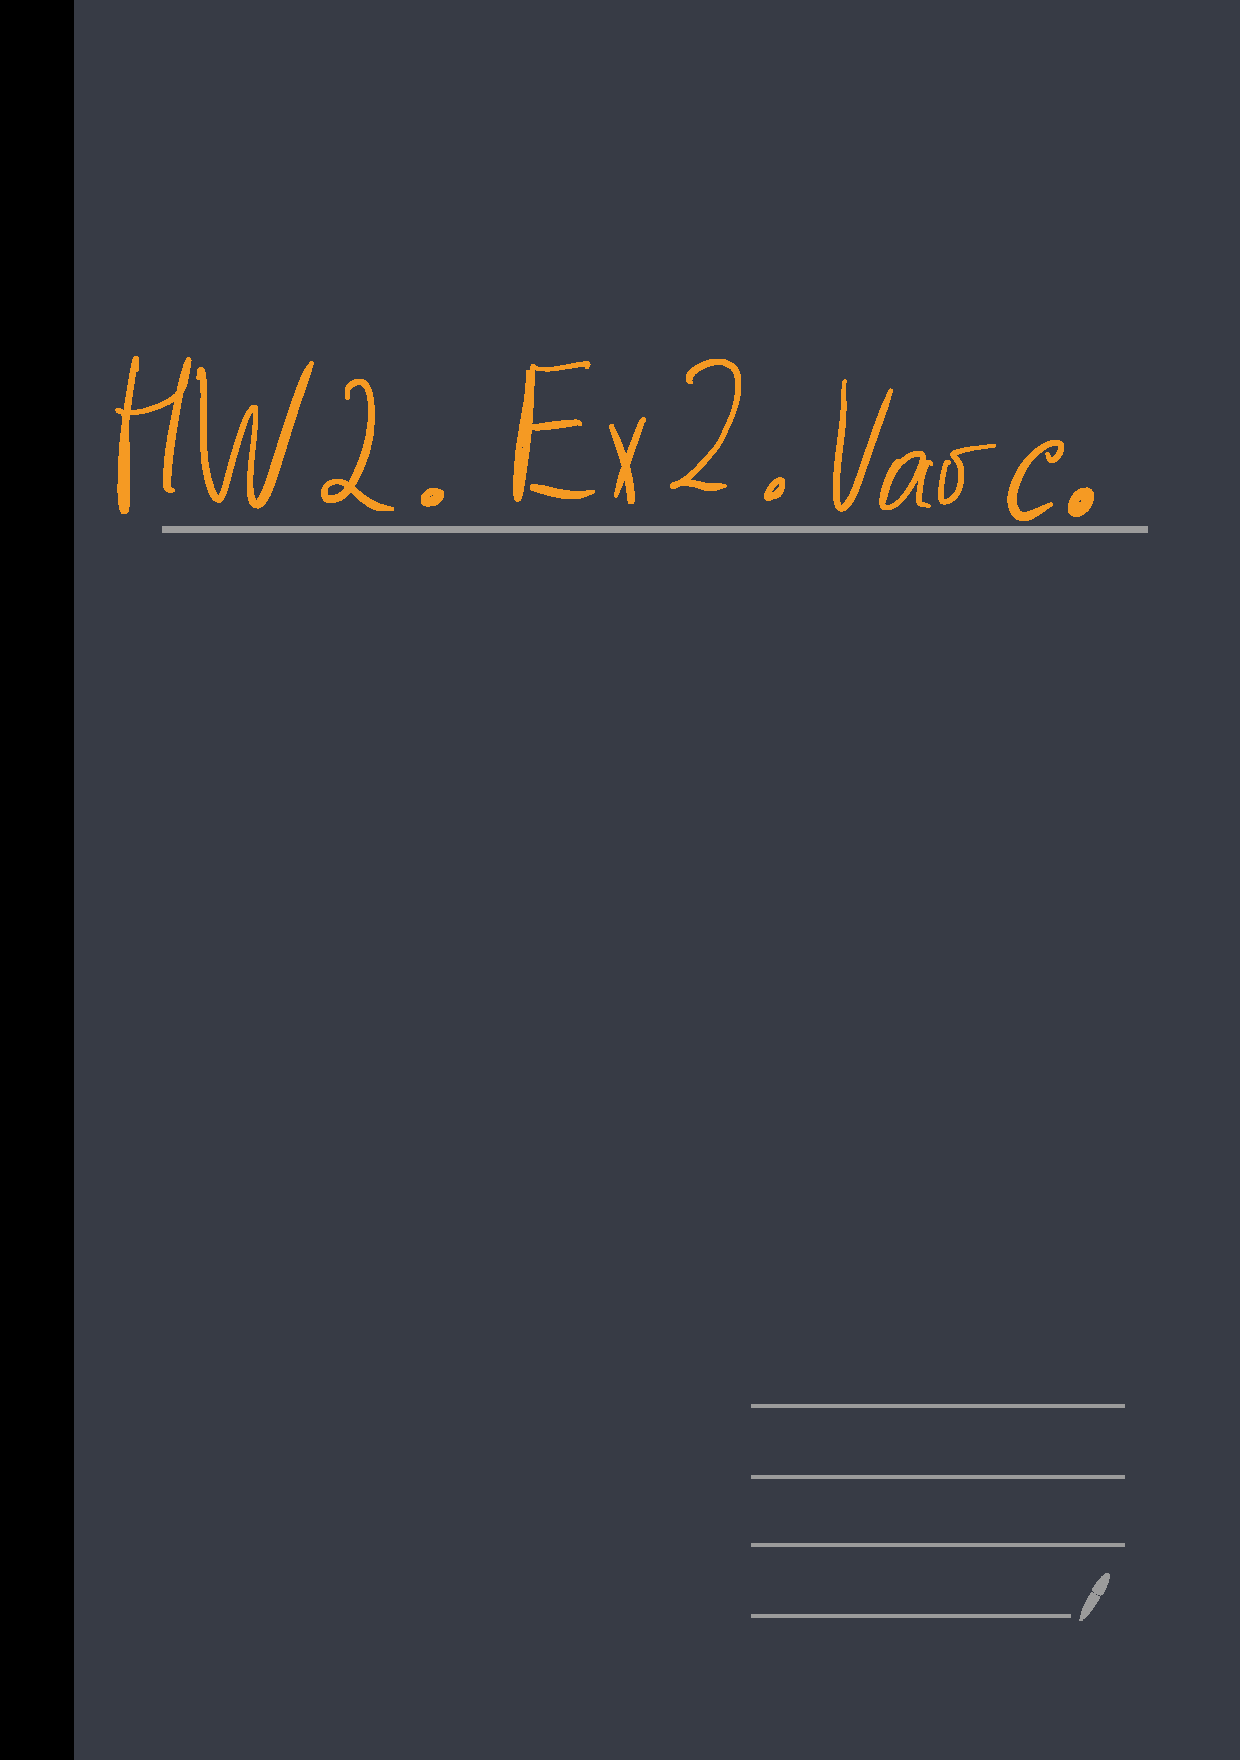
\includepdf[page={2}]{calculations/calc.pdf}
    
    \item On the figure \ref{fig:all} a scheme to compare input signal, simplified and original (shown at fig. \ref{fig:original}) systems' output is shown. 
    
        \begin{figure}[H]
            \centering
            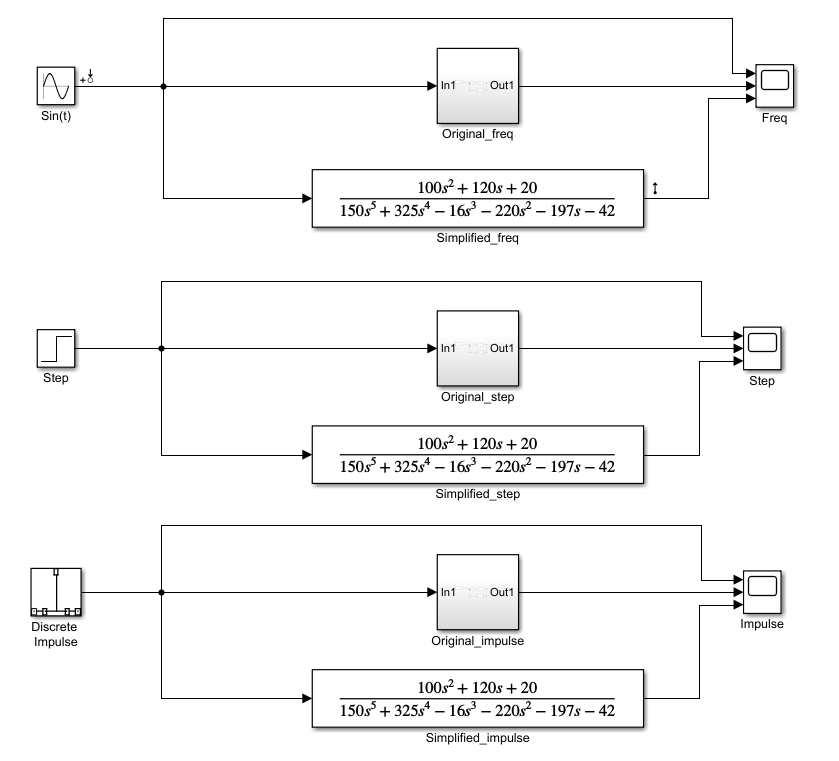
\includegraphics[width=15cm]{images/schemas/schemas.png}
            \caption{A schema for comparison original and simplified schema on different inputs}
            \label{fig:all}
        \end{figure}
    
    \begin{figure}[H]
            \centering
            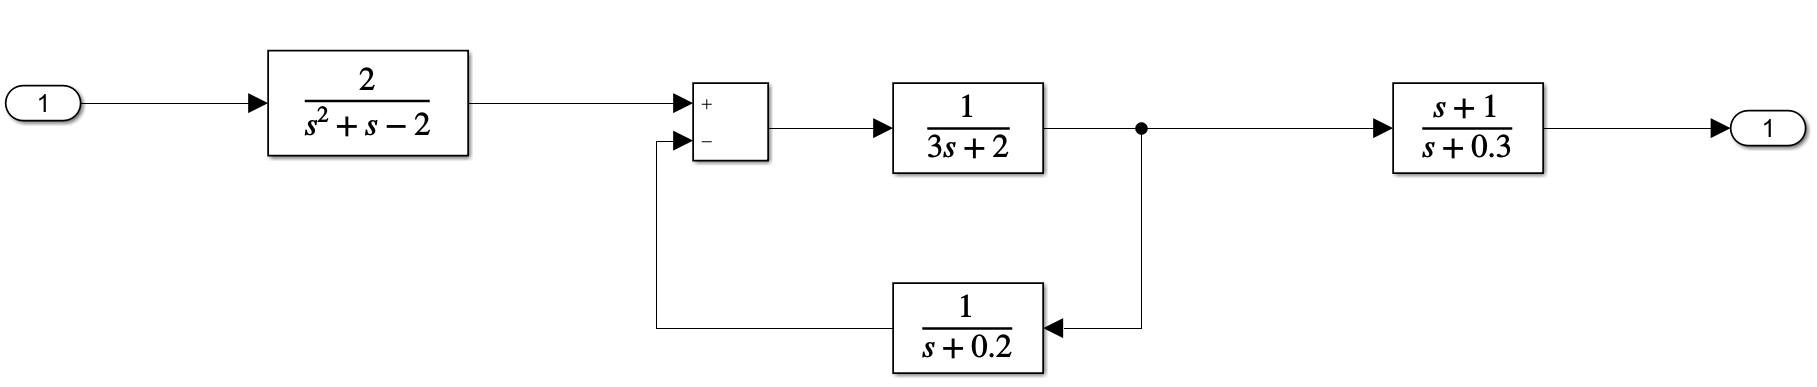
\includegraphics[width=15cm]{images/schemas/ex2_original.png}
            \caption{A sub-module containing the original schema}
            \label{fig:original}
        \end{figure}
    
    The graphs showing system's behaviour on different inputs are depicted on figures: 
    \begin{itemize}
        \item \ref{fig:sin_out} for frequency input;
        \item \ref{fig:step_out} for step input;
        \item \ref{fig:impulse_out} for impulse.
    \end{itemize}
    For all of 3 given inputs the system is unstable (will be formally proven further).

        
    \begin{figure}[H]
        \centering
        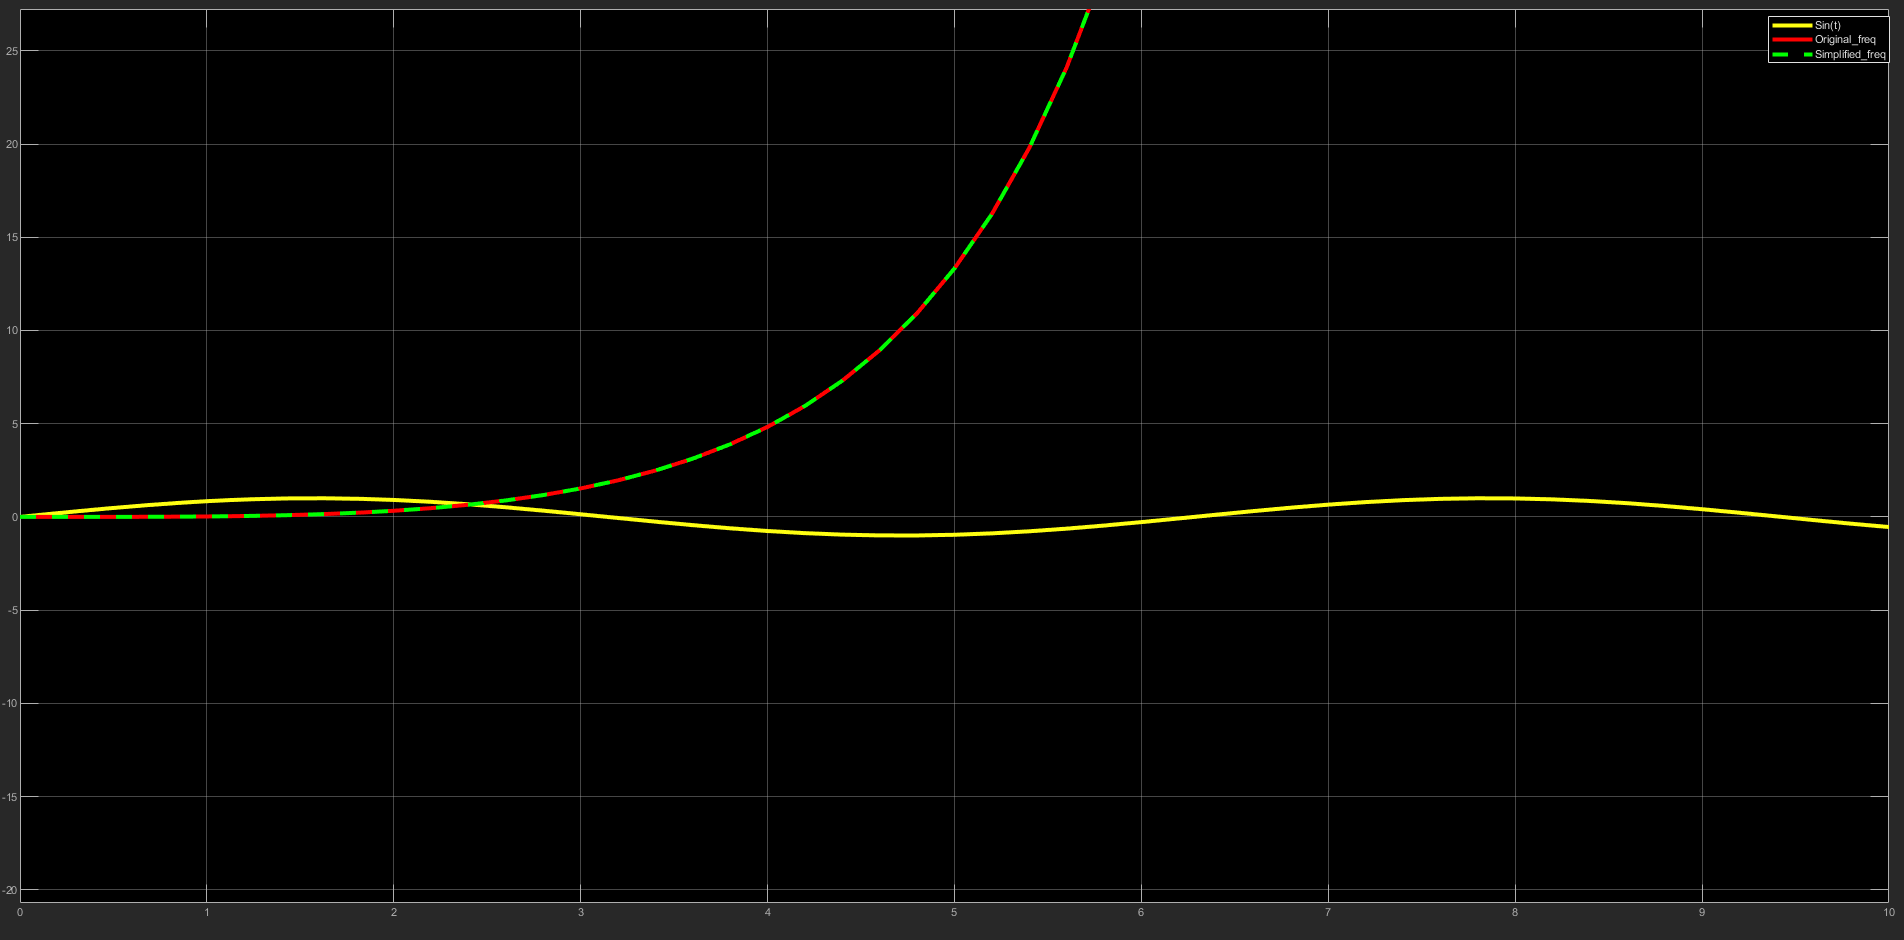
\includegraphics[width=15cm]{images/output/sin_out.png}
        \caption{A response for frequency input.}
        \label{fig:sin_out}
    \end{figure}
    
    \begin{figure}[H]
        \centering
        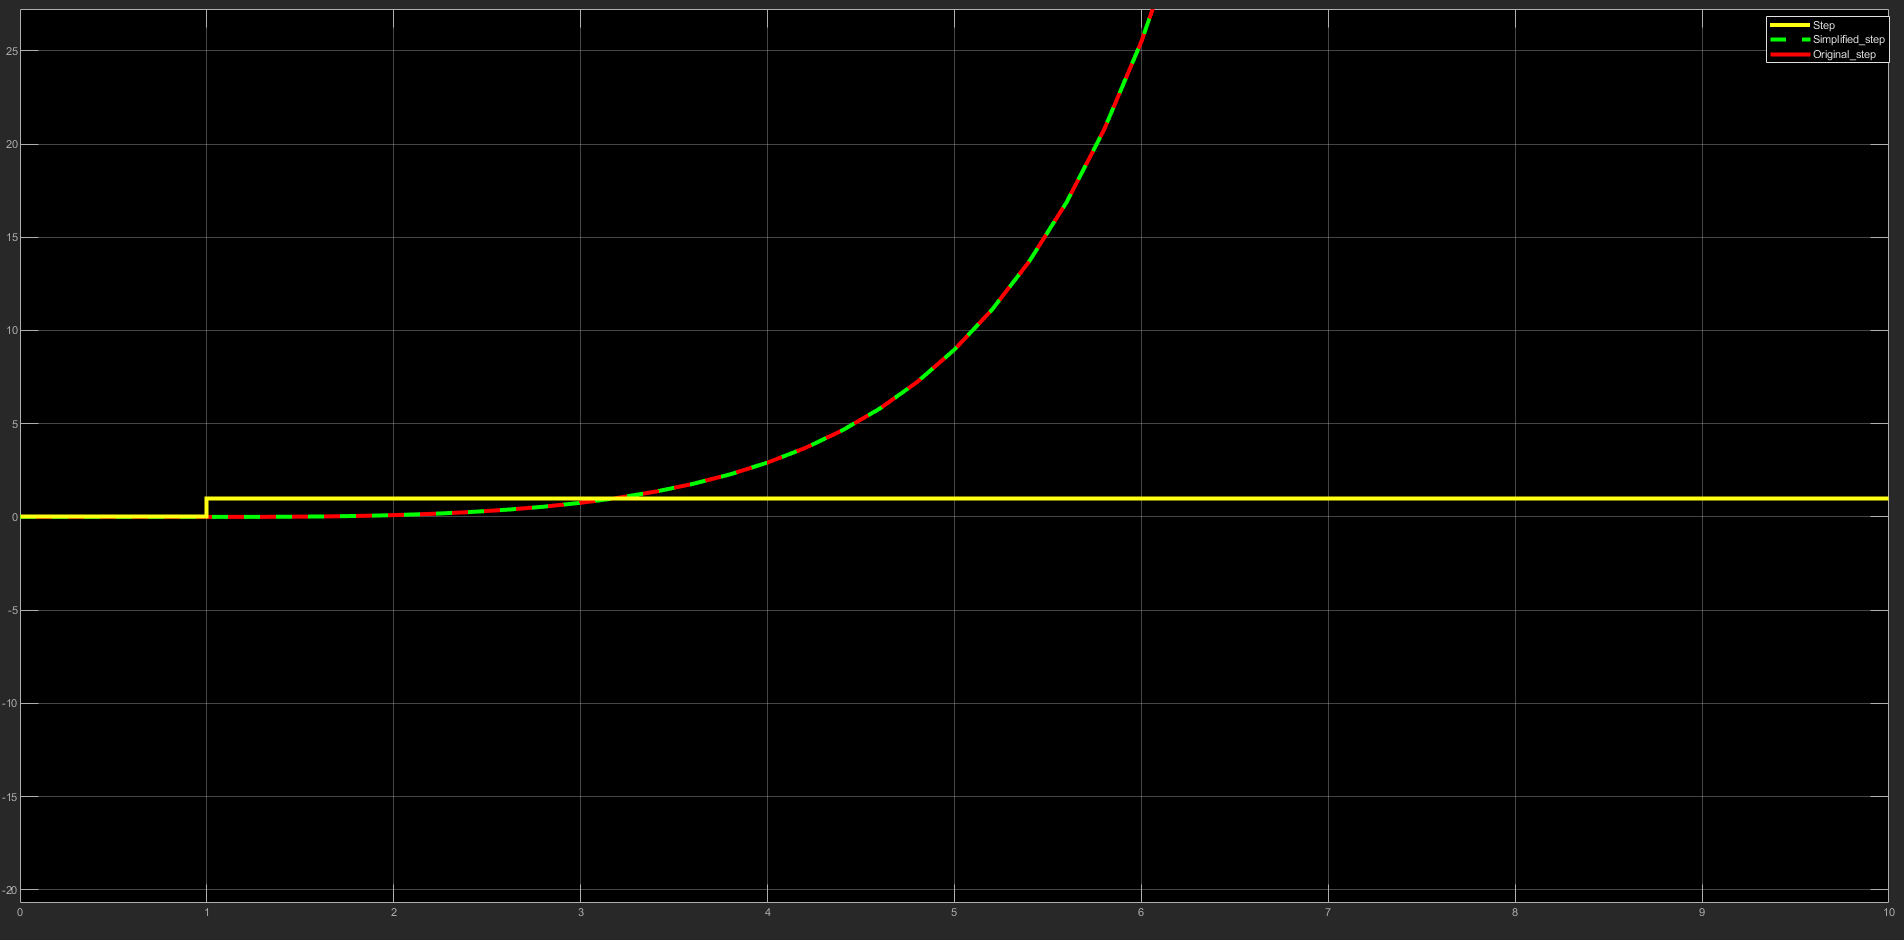
\includegraphics[width=15cm]{images/output/step_out.png}
        \caption{A response for step input.}
        \label{fig:step_out}
    \end{figure}
    
    \begin{figure}[H]
        \centering
        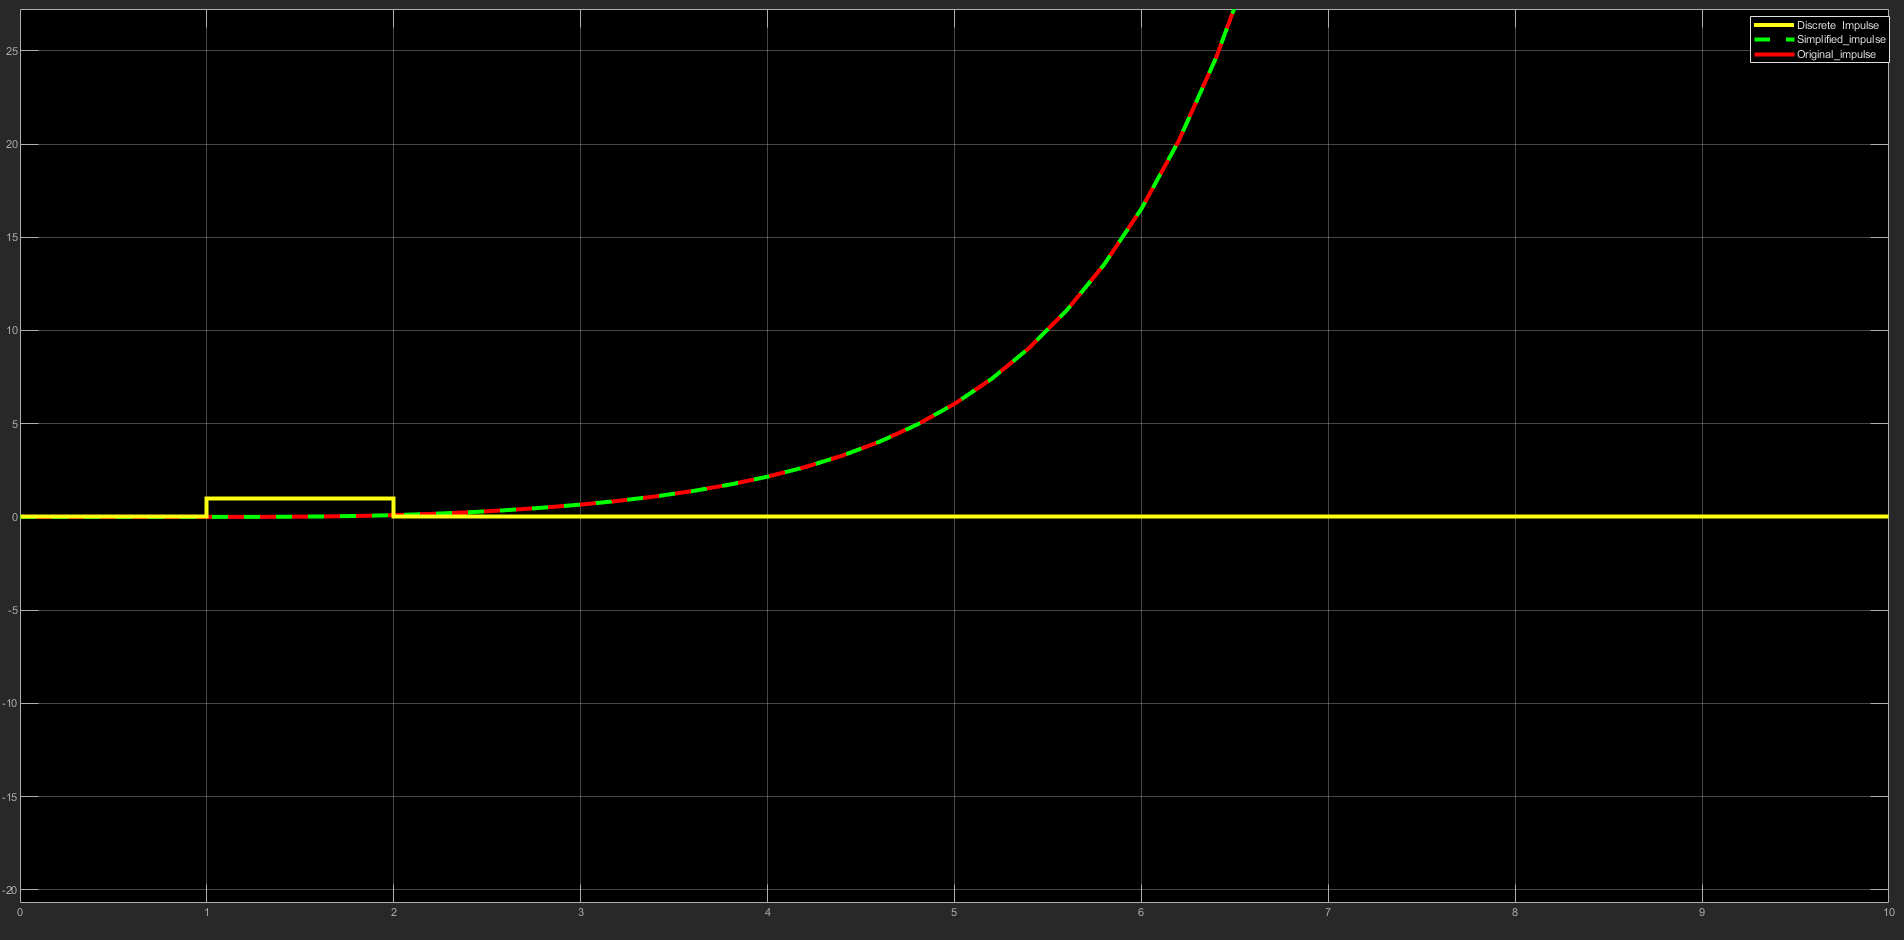
\includegraphics[width=15cm]{images/output/impulse_out.png}
        \caption{A response for impulse input.}
        \label{fig:impulse_out}
    \end{figure}
    
    \item Figures \ref{fig:zeroes} and \ref{fig:poles} show pole-zero map for frequency input. 
    
    \begin{subequations}
    \begin{tabularx}{\textwidth}{Xp{2cm}X}
        Zeroes:
        \begin{equation*}
             \begin{cases}
                s = -1\\
                s = - \frac{1}{5}
            \end{cases}
        \end{equation*}
        & &
        Poles:
        \begin{equation*}
            \begin{cases}
                s = -2\\
                s = - \frac{3}{10}\\
                s = 1\\
                s = \frac{1}{30}(-13 \pm i\sqrt{251})
            \end{cases}
        \end{equation*}
      \end{tabularx}
    \end{subequations}
    
    There is a pole at (1; 0), which makes the system unstable (Re > 0).
    
     \begin{figure}[H]
        \centering
        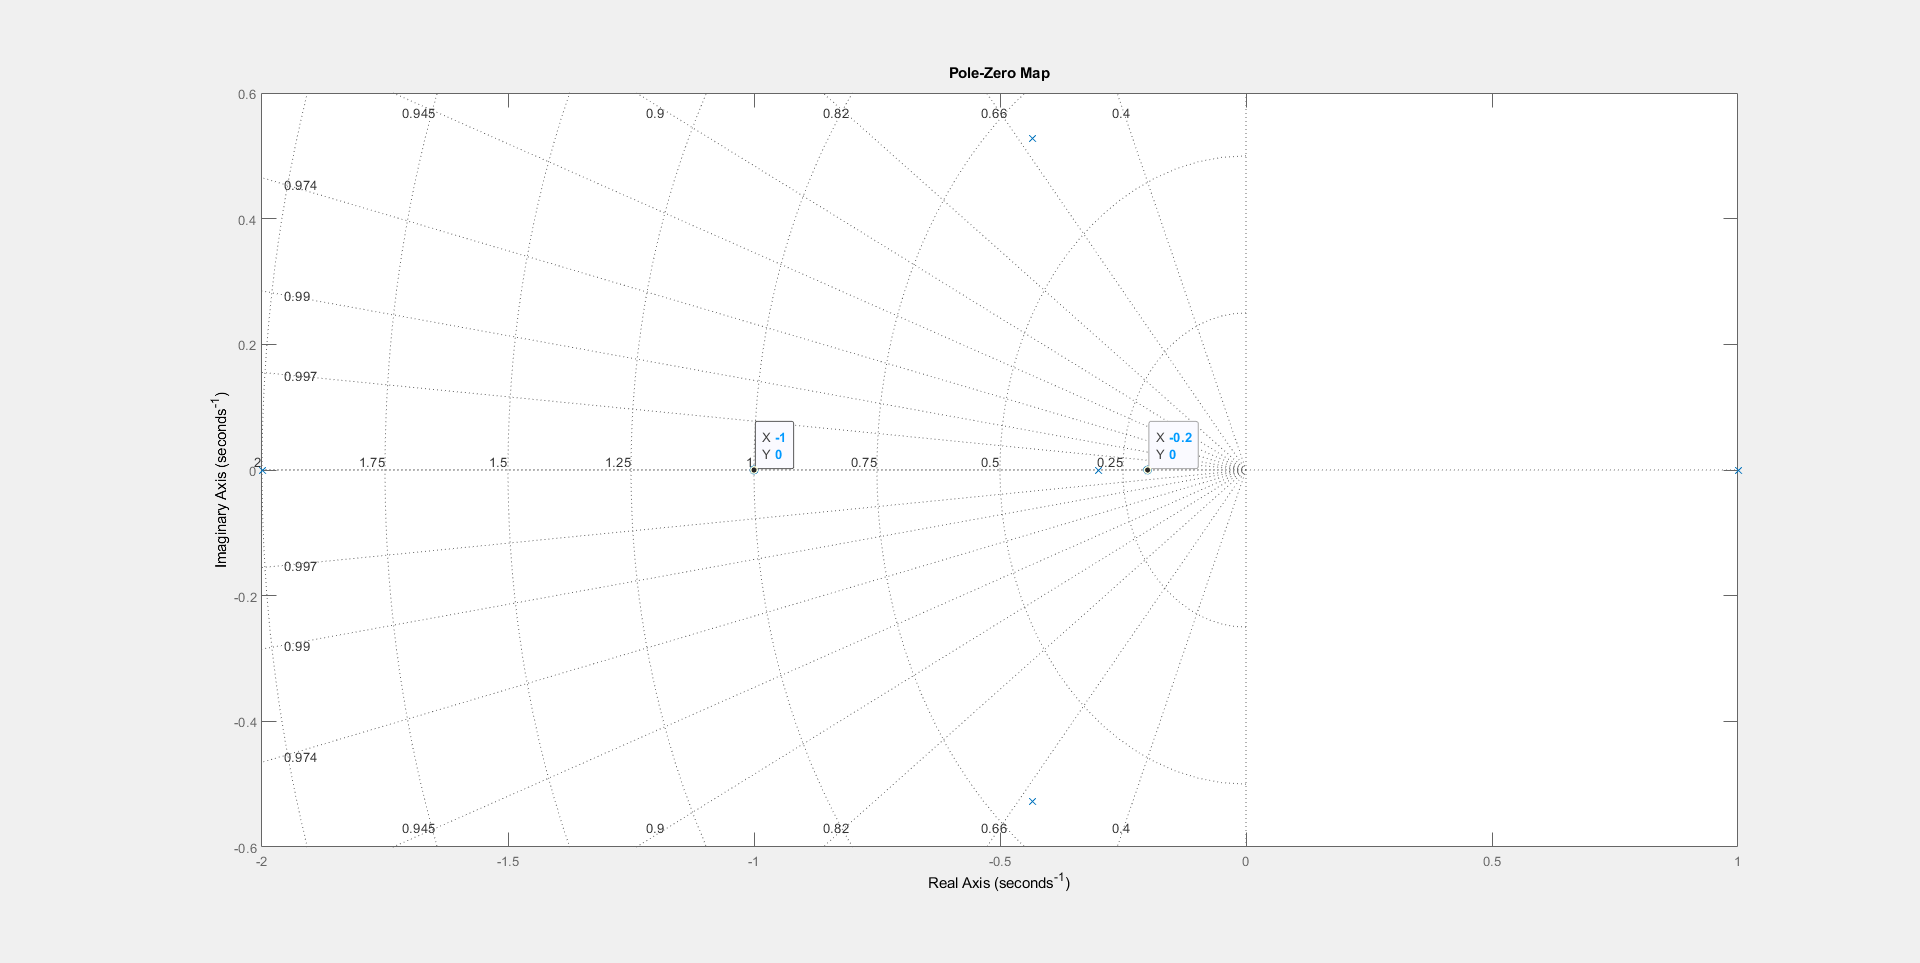
\includegraphics[width=15cm]{images/output/zero_sin.png}
        \caption{Pole-zero map with zeroes marked.}
        \label{fig:zeroes}
    \end{figure}
    
    \begin{figure}[H]
        \centering
        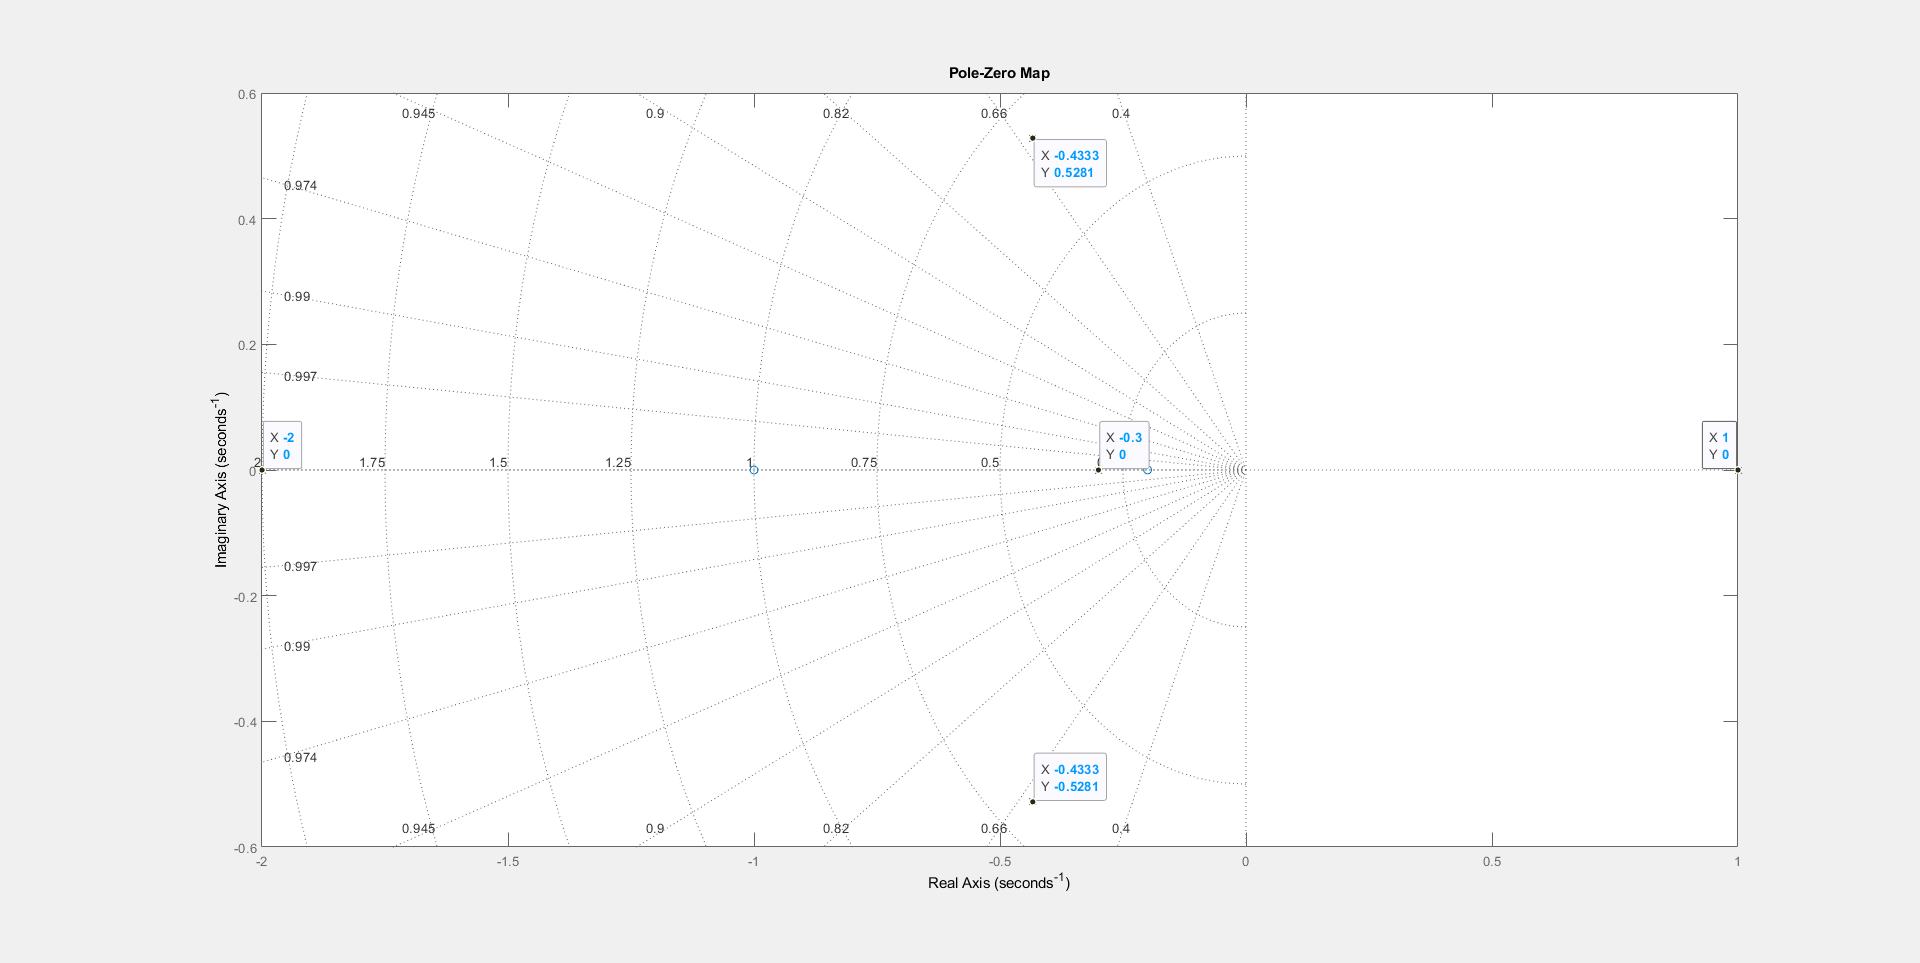
\includegraphics[width=15cm]{images/output/poles_sin.png}
        \caption{Pole-zero map with poles marked.}
        \label{fig:poles}
    \end{figure}
    
    \item Figure \ref{fig:bode} shows the Bode plot. \\
    The phase graph intersects $-180$ at  frequency = $0.322$ $rad/sec$, value of magnitude at this point is a gain margin $\approx 4.17$ $dB$. The magnitude graph never intersect 0, thus the phase margin is $\infty$.
    
    Let's calculate asymptotes:
    \begin{enumerate}
        \item 
        \begin{equation*}
            \frac{100s^2+120s+20}{150s^5+325s^4-16s^3-220s^2-197s-42} = 
            - \frac{20}{42} \frac{5s^2+6s+1}{-\frac{150}{42}s^5 - \frac{325}{42}s^4 + \frac{16}{42}s^3 + \frac{220}{42}s^2 + \frac{197}{42}s + 1}
        \end{equation*}
        Thus the graph starts at magnitude $-20\log_{10}\left(\frac{20}{42}\right) = -6.44dB$ at phase $-180\degree$ with zero growth rate($\Delta = 0$).
        
        \item Then we consider a pole $-2$ which produces a break frequency $10^{-1}$ $rad/sec$. The magnitude starts to decrease at rate $\Delta = -20$ $dB/dec$ up to zero $-1$.
        
        \item A zero $-1$ increases grow rate by $20$ $dB/dec$, so overall rate become $\Delta = 0$ $dB/dec$ up to next pole
        
        \item The next pole is a pair of complex-conjugate roots at $Re(\dots) = -\frac{13}{30}$, that decreases overall rate by $40$ $dB/dec$ resulting in $\Delta = -40$ $dB/dec$
        
        \item Following critique point is a pole at $-0.3$ which will reduce growing by $20$ $dB/dec$, thus having $\Delta = -60$ $dB/dec$
        
        \item Zero at $-2$ will increase growth rate resulting in $\Delta = -40$ $dB/dec$
        
        \item Finally a pole at $1$ will decrease a rate, so after this point $\Delta = - 60$ $dB/dec$
    \end{enumerate}
    As we can see, the majority of growth rate changes happen between $-2$ and $1$ which is a very small interval compared to logarithmic scale.
    
    \begin{figure}[H]
        \centering
        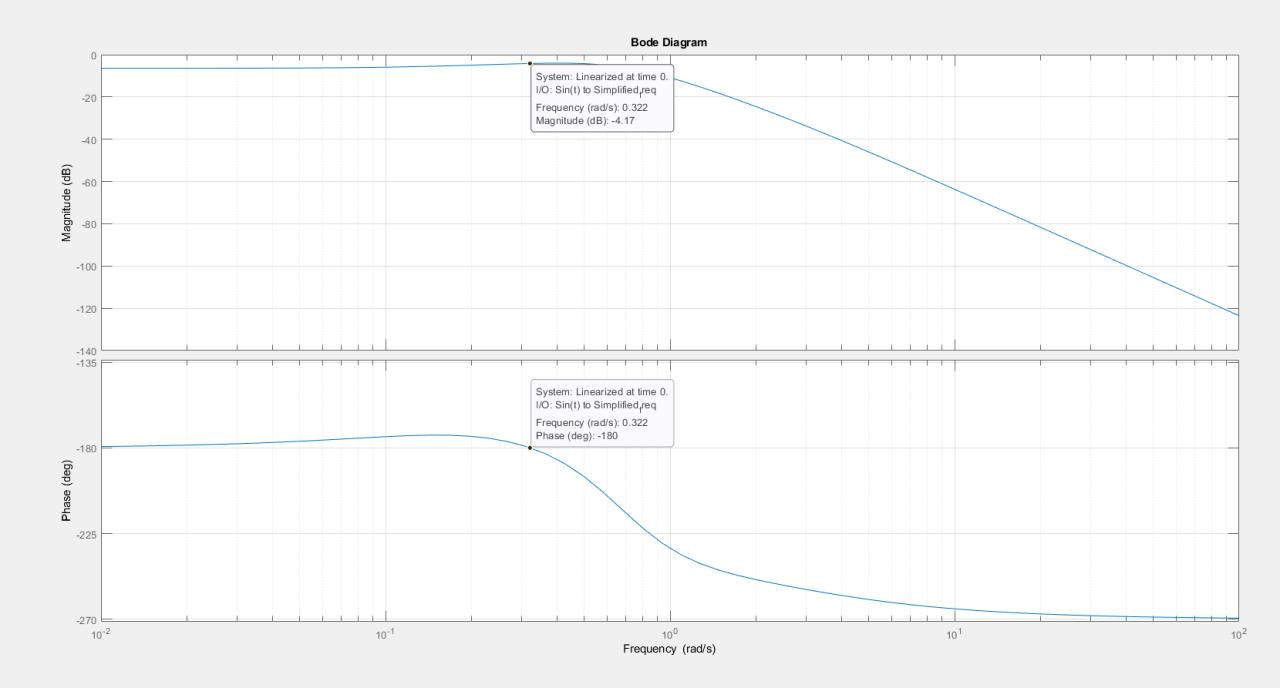
\includegraphics[width=15cm]{images/output/bode.jpg}
        \caption{Bode plot.}
        \label{fig:bode}
    \end{figure}
    
\end{enumerate}

\section*{Question 3}
\label{Q:3}
\textit{Step-by-step calculations are present on the following page} \\
Given: \\
\begin{subequations}
  \begin{tabularx}{\textwidth}{Xp{2cm}X}
  \begin{equation*}
     W(s) = \frac{s+4}{3s+2}
  \end{equation*}
  & &
  \begin{equation*}
    M(s) = \frac{1}{s+1}
  \end{equation*}
  \end{tabularx}
\end{subequations}
\begin{enumerate}[leftmargin=!,labelindent=5pt]
    \item Transfer function for $g(t)$, given $f(t) = 0$:
    \begin{equation*}
        W_{xg} = \frac{W}{1+W} = \frac{s+4}{4s+6}
    \end{equation*}
    
     \item Transfer function for $f(t)$, given $g(t) = 0$:
    \begin{equation*}
        W_{xf} = \frac{M}{1 + W} = \frac{3s+2}{4s^2 + 10s + 6}
    \end{equation*}
    
    \item Total transfer function:
    \begin{align*}
        x &= W_{xg}(s)g(t) + W_{xf}(s)f(t)\\ &= \frac{s+4}{4s+6} * g(t) + \frac{3s+2}{4s^2 + 10s + 6} * f(t)
    \end{align*}
    
    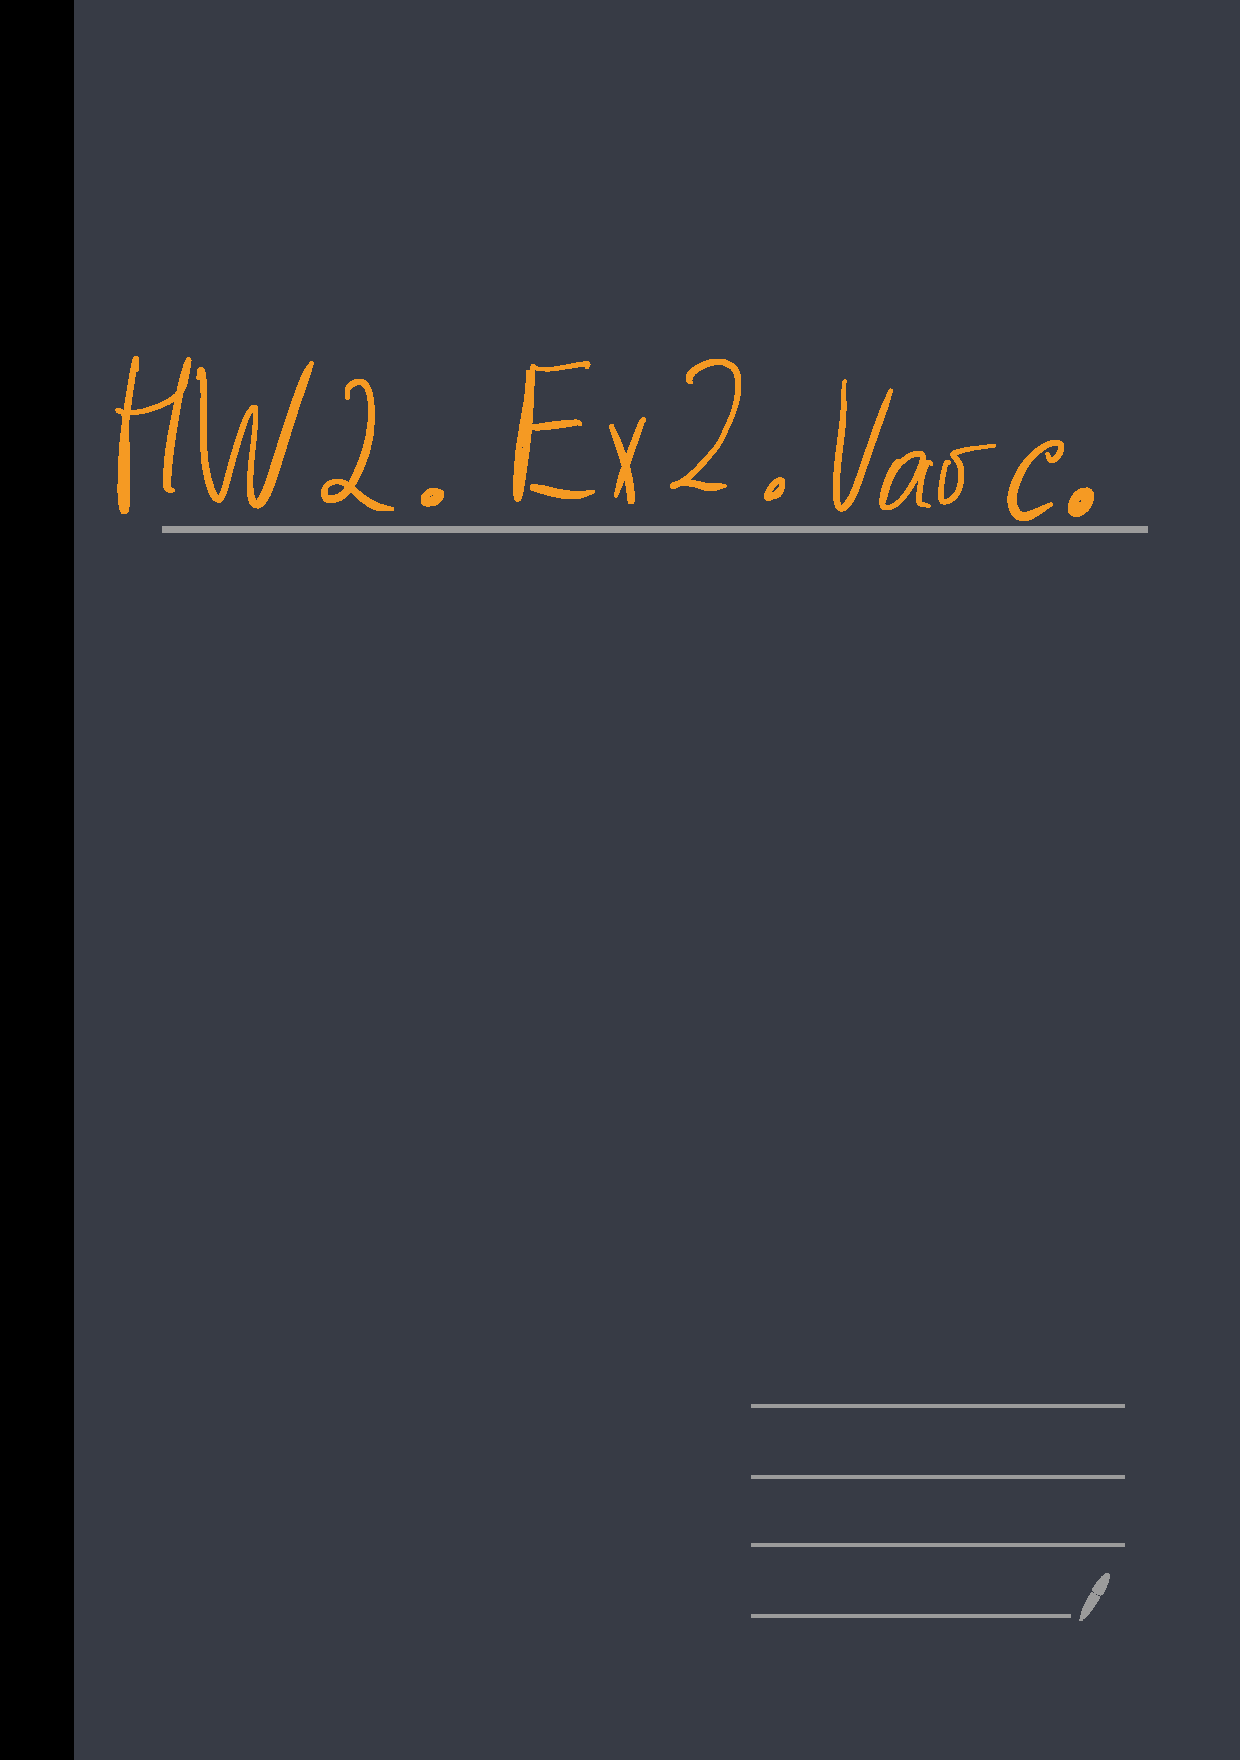
\includepdf[page={4}]{calculations/calc.pdf}
\end{enumerate}

\section*{Question 4}
\label{Q:4}

Find transfer function of the system: \\ 
\begin{subequations}
  \begin{tabularx}{\textwidth}{Xp{2cm}X}
  \begin{equation*}
    A = \left( \begin{matrix} 2 & 0 \\ -3 & 1 \end{matrix} \right)
  \end{equation*}
  & &
  \begin{equation*}
   B = \left( \begin{matrix} -1 \\ 1 \end{matrix} \right)
  \end{equation*}
  \\
  \begin{equation*}
   C = \left( \begin{matrix} -2 & 0 \end{matrix} \right)
  \end{equation*}
  & &
  \begin{equation*}
   D =  \left( \begin{matrix} 2 \end{matrix} \right)
  \end{equation*}
  \end{tabularx}
\end{subequations}
\setcounter{equation}{0}
 We know, that the transfer function for a SS is: $C(sI-A)^{-1}B+D$.

 \begin{equation}\label{eq:1}
    sI - A = \left( \begin{matrix} s-2 & 0 \\ 3 & s-1 \end{matrix} \right) 
 \end{equation}
 
Since matrix obtained after step \eqref{eq:1} is 2x2, we can find it's inverse according to the following formula:
\begin{equation*}
    \left( \begin{matrix} a & b \\ c & d \end{matrix} \right)^{-1} = 
        \frac{1}{ad-cb}  \left( \begin{matrix} d & -b \\ -c & a \end{matrix} \right)
\end{equation*}

Thus
 \begin{align*}
    (sI - A)^{-1} &= \frac{1}{s^2-3s+2} \left( \begin{matrix} s-1 & 0 \\ -3 & s-2 \end{matrix} \right) \\
    (sI - A)^{-1}B &= \frac{1}{s^2-3s+2} \left( \begin{matrix} s-1 & 0 \\ -3 & s-2 \end{matrix} \right) \cdot \left( \begin{matrix} -1 \\ 1 \end{matrix} \right) \\
    &= \frac{1}{s^2-3s+2} \left( \begin{matrix} 1-s \\ s+1 \end{matrix} \right) \\
    C(sI - A)^{-1}B &= \frac{1}{s^2-3s+2} \left( \begin{matrix} -2 & 0 \end{matrix} \right) \cdot
    \left( \begin{matrix} 1-s \\ s+1 \end{matrix} \right) \\
    &= \frac{2s - 2}{s^2-3s+2} \\
    C(sI - A)^{-1}B + D &= \frac{2s - 2}{s^2-3s+2} + 2 \\
    &= \frac{2s^2-4s+2}{s^2-3s+2}
 \end{align*}
 
 Answer: 
 \begin{equation*}
     W=\frac{2s^2-4s+2}{s^2-3s+2}
 \end{equation*}
 
\section*{Question 5}
\label{Q:5}

Find transfer function of the system: \\ 
\begin{subequations}
  \begin{tabularx}{\textwidth}{Xp{2cm}X}
  \begin{equation*}
    A = \left( \begin{matrix} 4 & 1 \\ -2 & 1 \end{matrix} \right)
  \end{equation*}
  & &
  \begin{equation*}
   B = \left( \begin{matrix} 2 & 1 \\ 3 & 0 \end{matrix} \right)
  \end{equation*}
  \\
  \begin{equation*}
   C = \left( \begin{matrix} 1 & 3 \end{matrix} \right)
  \end{equation*}
  & &
  \begin{equation*}
   D =  \left( \begin{matrix} 1 & 2 \end{matrix} \right)
  \end{equation*}
  \end{tabularx}
\end{subequations}
\setcounter{equation}{1}
 We know, that the transfer function for a SS is: $C(sI-A)^{-1}B+D$.

 \begin{equation}\label{eq:2}
    sI - A = \left( \begin{matrix} s-4 & -1 \\ 2 & s-1 \end{matrix} \right) 
 \end{equation}
 
Since matrix obtained after step \eqref{eq:2} is 2x2, we can find it's inverse according to the following formula:
\begin{equation*}
    \left( \begin{matrix} a & b \\ c & d \end{matrix} \right)^{-1} = 
        \frac{1}{ad-cb}  \left( \begin{matrix} d & -b \\ -c & a \end{matrix} \right)
\end{equation*}

Thus
 \begin{align*}
    (sI - A)^{-1} &= \frac{1}{s^2-5s+6} \left( \begin{matrix} s-1 & 1 \\ -2 & s-4 \end{matrix} \right) \\
    (sI - A)^{-1}B &= \frac{1}{s^2-5s+6} \left( \begin{matrix} s-1 & 1 \\ -2 & s-4 \end{matrix} \right) \cdot \left( \begin{matrix} 2 & 1 \\ 3 & 0 \end{matrix} \right) \\
    &= \frac{1}{s^2-5s+6} \left( \begin{matrix} 2s+1 & s-1 \\ 3s-16 & -2 \end{matrix} \right) \\
    C(sI - A)^{-1}B &= \frac{1}{s^2-5s+6} \left( \begin{matrix} 1 & 3 \end{matrix} \right) \cdot \left( \begin{matrix} 2s+1 & s-1 \\ 3s-16 & -2 \end{matrix} \right) \\
    &= \frac{1}{s^2-5s+6} \left( \begin{matrix} 11s - 47 & s-7 \end{matrix} \right) \\
    C(sI - A)^{-1}B + D &= \frac{1}{s^2-5s+6} \left( \begin{matrix} 11s - 47 & s-7 \end{matrix} \right) +   \left( \begin{matrix} 1 & 2 \end{matrix} \right)\\
    &= \frac{1}{s^2-5s+6} \left( \begin{matrix} 11s - 46 & s-5 \end{matrix} \right)
 \end{align*}
 
 Answer: 
\begin{equation*}
    \begin{cases}
        W_1 = \frac{11s-46}{s^2-5s+6} \\
        W_2 = \frac{s-5}{s^2-5s+6}
    \end{cases}
\end{equation*}


\section*{Question 6}
\label{Q:6}
\textit{Step-by-step calculations are present on the following page}
\begin{enumerate}[leftmargin=!,labelindent=5pt]
    \item Transfer function for $f$, given $x = 0$:
    \begin{equation*}
        W_{yf} = \frac{W_3 W_5 W_6 W_7}{1 - W_4 W_6 - W_2 W_3 W_5 W_6}
    \end{equation*}
    
    \item Transfer function for $x$, given $f = 0$:
    \begin{equation*}
        W_{yx} = \frac{W_1 + W_3 W_8}{W_3} * \frac{W_3 W_5 W_6 W_7}{1 - W_4 W_6 - W_2 W_3 W_5 W_6}
    \end{equation*}
    
    \item Finally:
    \begin{align*}
        y &=  W_{yf} * f(t) +  W_{xf} * x(t) \\
        &= \frac{W_3 W_5 W_6 W_7}{1 - W_4 W_6 - W_2 W_3 W_5 W_6} * f(t) + \frac{W_1 + W_3 W_8}{W_3} * \frac{W_3 W_5 W_6 W_7}{1 - W_4 W_6 - W_2 W_3 W_5 W_6} * x(t)
    \end{align*}
    
    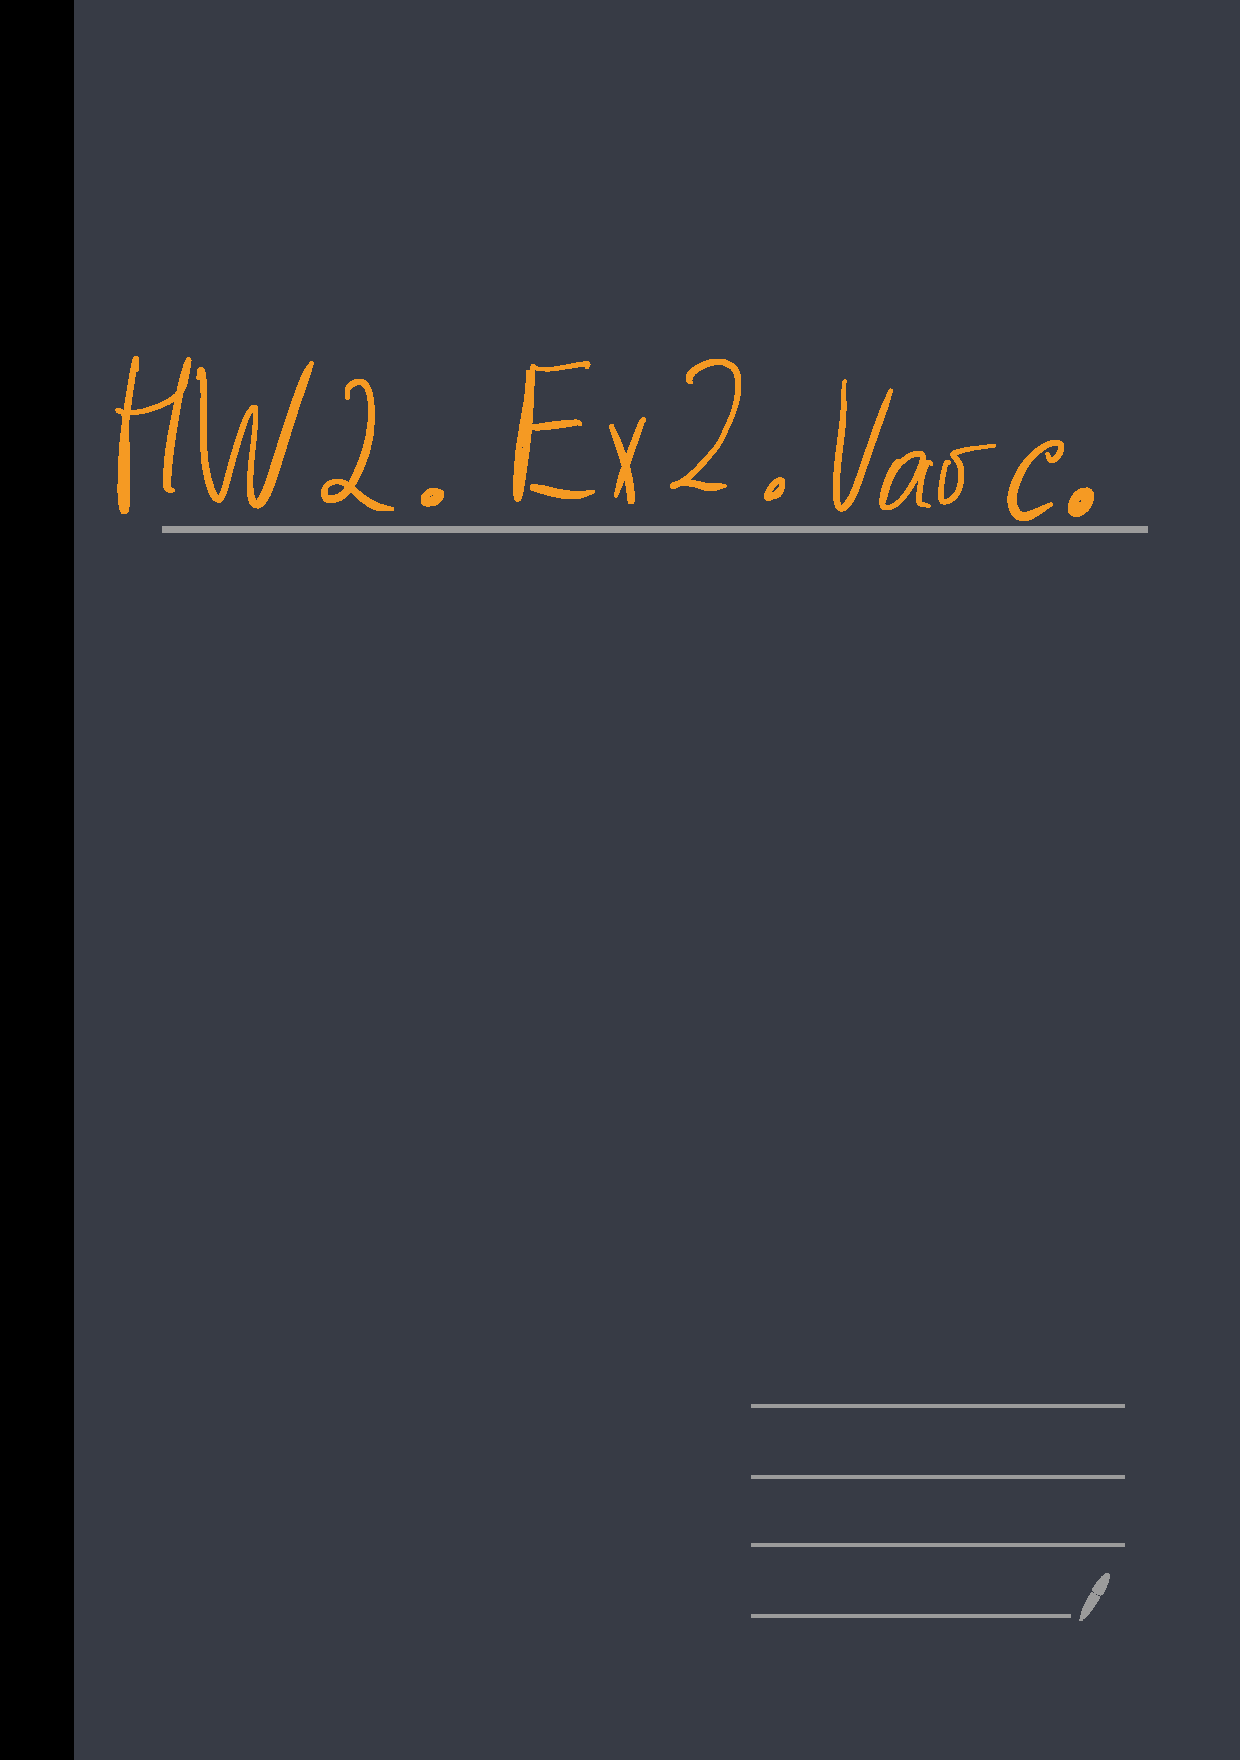
\includepdf[page={6,7}]{calculations/calc.pdf}
\end{enumerate}
\end{document}
